\section{Considering Contaminant Transport Mechanism}


\begin{frame}
  \frametitle{Indicators, Tracers, and Surrogates}
  \begin{block}{Idea}
    \begin{itemize}
      \item Use some ITS to predict period when VI is most significant
      \item Building pressurization good for advection site - determine using weather?
    \end{itemize}
  \end{block}
\end{frame}


\begin{frame}
  \frametitle{Predicting Building Pressurization}
  \begin{figure}
    \centering
    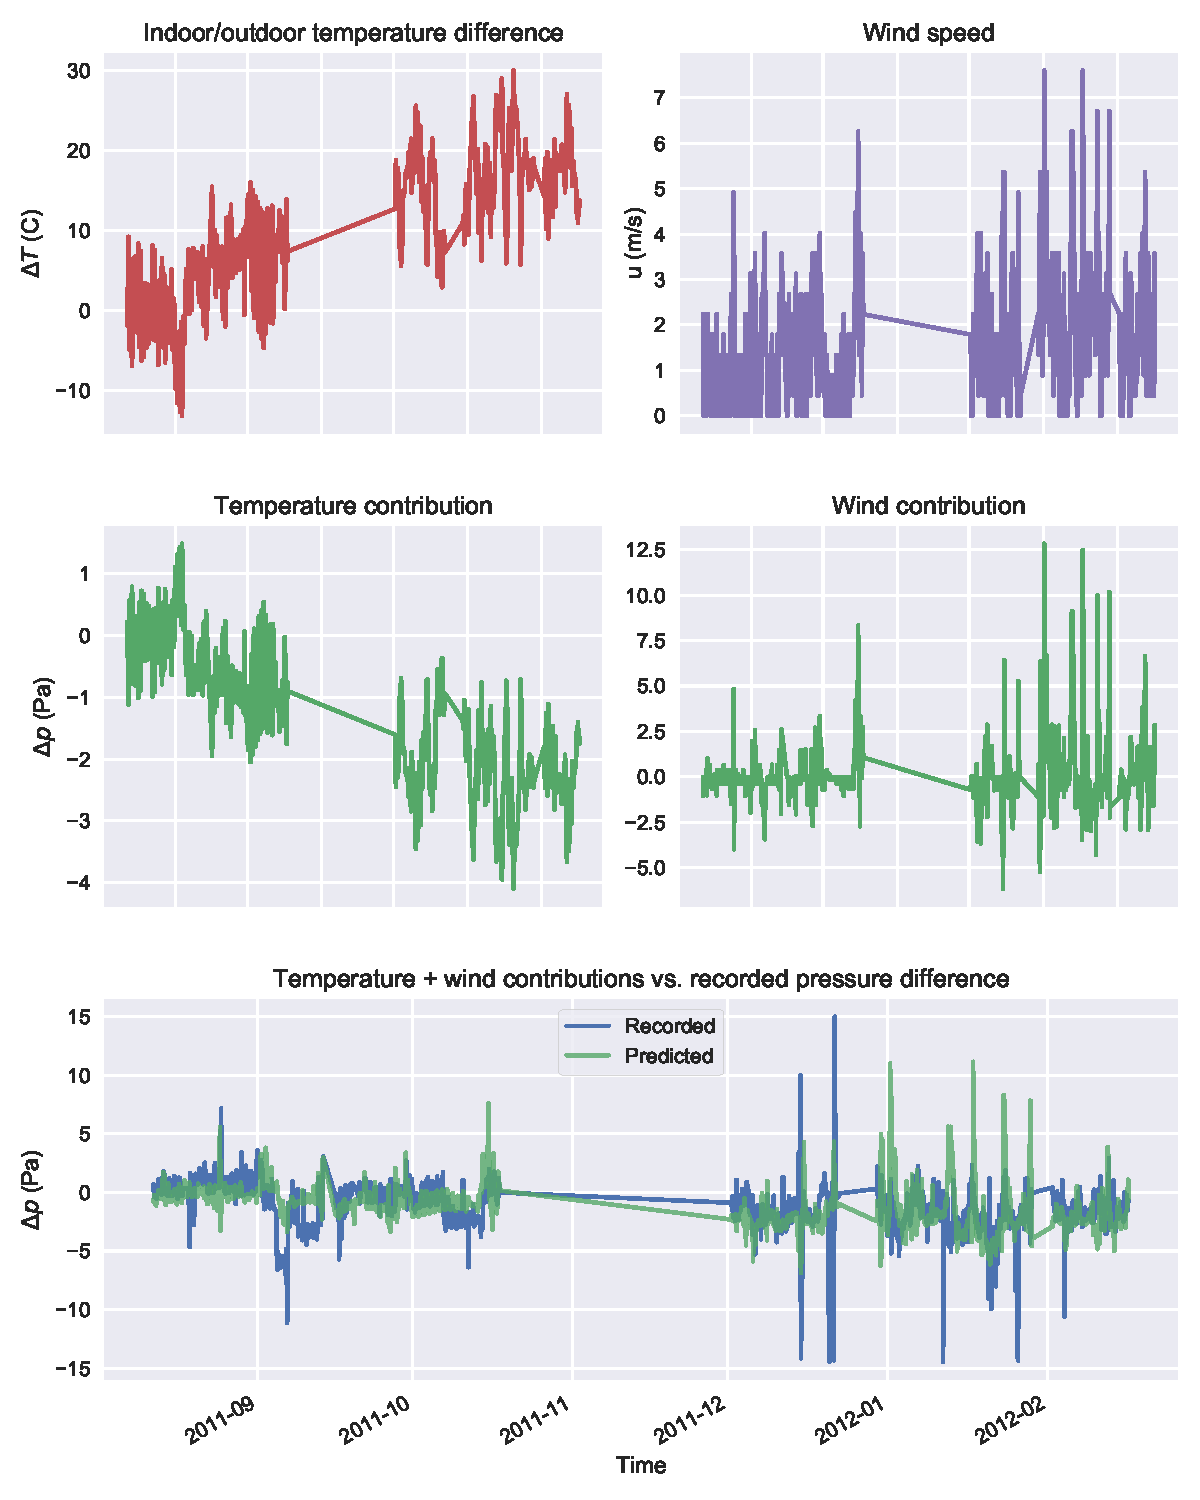
\includegraphics[height=0.8\textheight]{pressure_prediction.pdf}
  \end{figure}
\end{frame}

\begin{frame}
  \frametitle{Predicting Building Pressurization}
  \begin{figure}
    \centering
    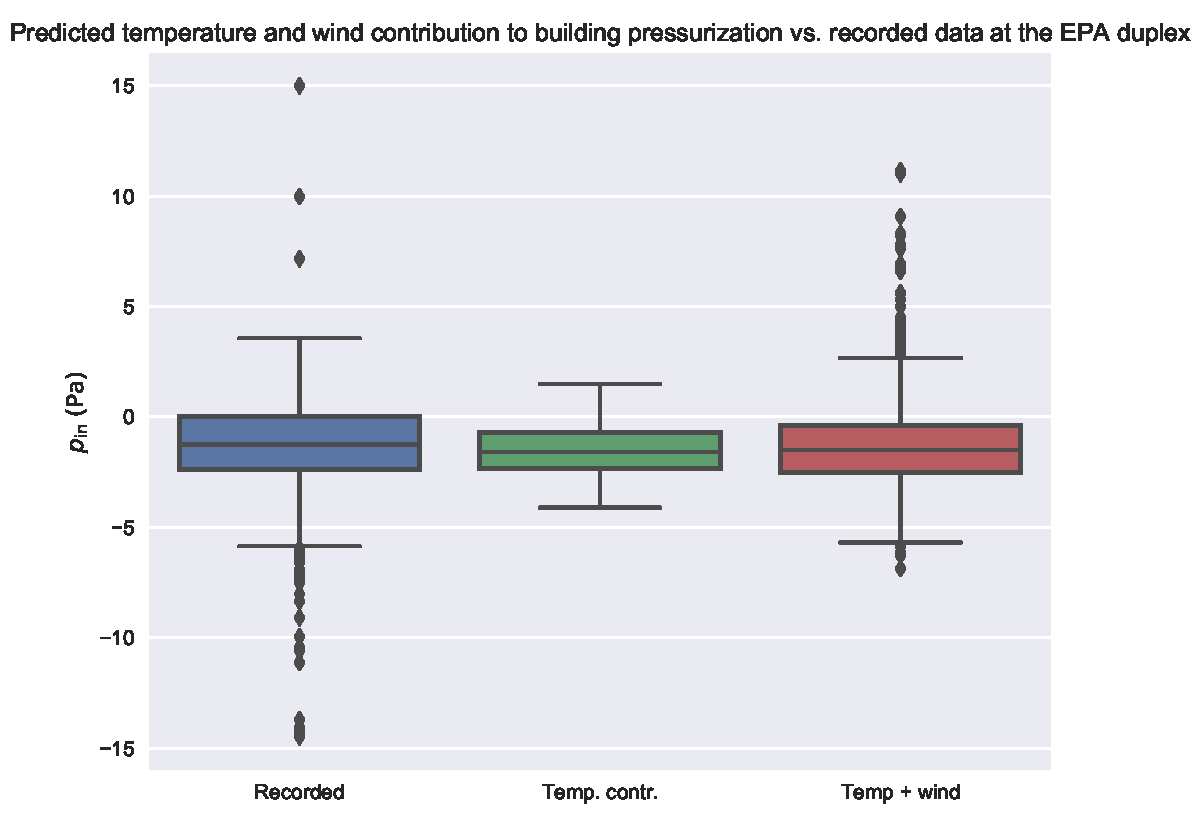
\includegraphics[width=\textwidth]{pressure_prediction_boxplot.pdf}
  \end{figure}
\end{frame}

\begin{frame}
  \frametitle{Seasonal Pressure}
  \begin{figure}
    \centering
    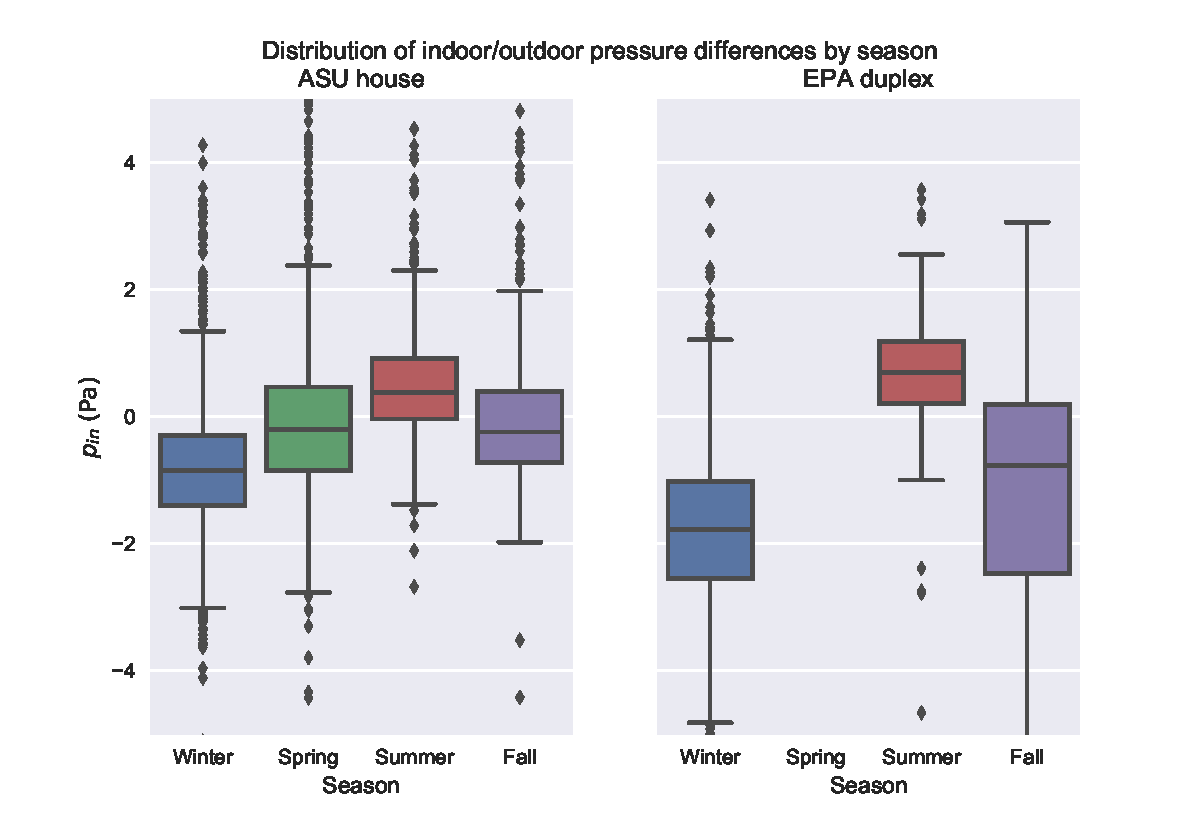
\includegraphics[width=\textwidth]{seasonal_pressure.pdf}
  \end{figure}
\end{frame}

\begin{frame}
  \frametitle{Seasonal Indoor Contaminant Concentration}
  \begin{figure}
    \centering
    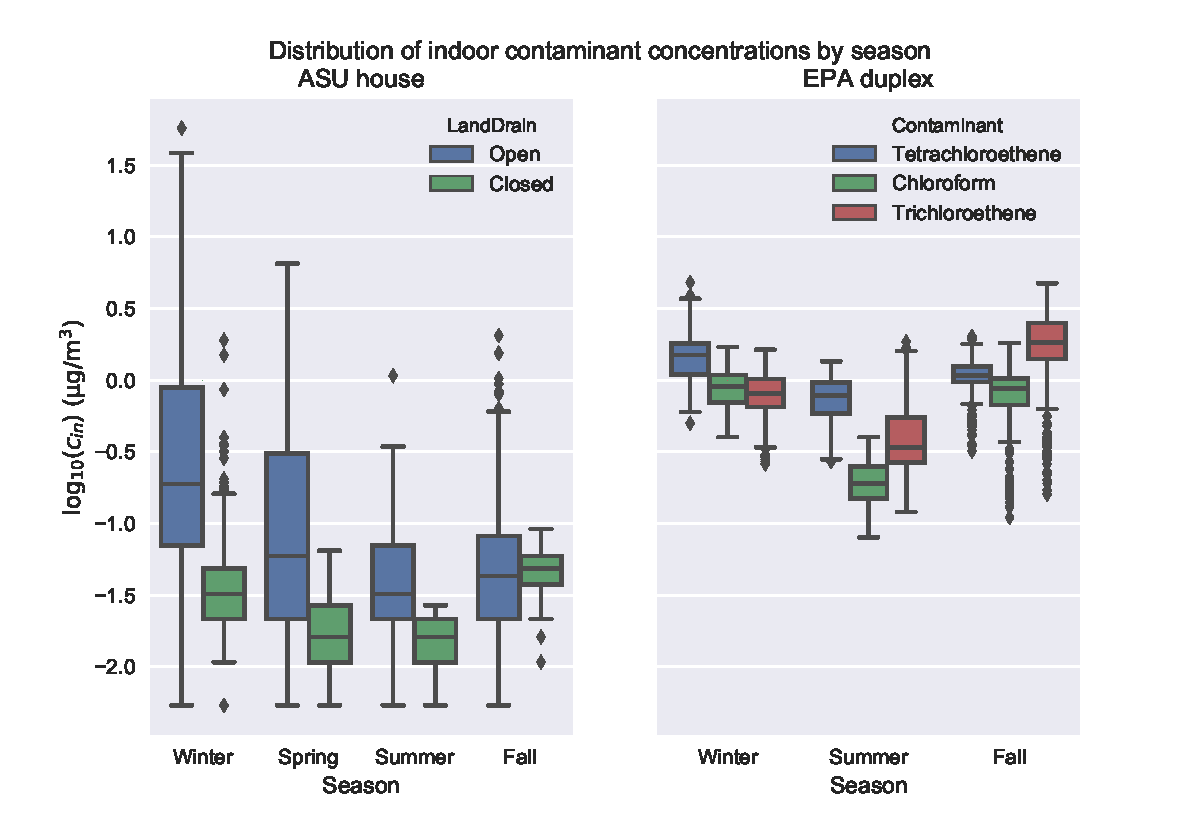
\includegraphics[width=\textwidth]{seasonal_concentration.pdf}
  \end{figure}
\end{frame}

\begin{frame}
  \begin{alertblock}{Key insights}
    \begin{itemize}
      \item Building pressurization can quite easily be predicted using weather conditions
      \item For sites dominated by advective contaminant entry building pressurization can be an effective ITS
    \end{itemize}
  \end{alertblock}
\end{frame}
